% Created 2019-01-10 jue 13:02
% Intended LaTeX compiler: pdflatex
\documentclass[xcolor={usenames,svgnames,dvipsnames}]{beamer}
\usepackage[utf8]{inputenc}
\usepackage[T1]{fontenc}
\usepackage{graphicx}
\usepackage{grffile}
\usepackage{longtable}
\usepackage{wrapfig}
\usepackage{rotating}
\usepackage[normalem]{ulem}
\usepackage{amsmath}
\usepackage{textcomp}
\usepackage{amssymb}
\usepackage{capt-of}
\usepackage{hyperref}
\usepackage{color}
\usepackage{listings}
\usepackage[spanish]{babel}
\usecolortheme{rose}
\setbeamercolor{alerted text}{fg=Blue}
\setbeamerfont{alerted text}{series=\bfseries}
\setbeamercolor{block title}{bg=structure.fg!20!bg!50!bg}
\setbeamercolor{block body}{use=block title,bg=block title.bg}
\setbeamertemplate{navigation symbols}{}
\AtBeginSection[]{\begin{frame}[plain]\tableofcontents[currentsection,hideallsubsections]\end{frame}}
\AtBeginSubsection[]{\begin{frame}[plain]\tableofcontents[currentsubsection,sectionstyle=show/shaded,subsectionstyle=show/shaded/hide]\end{frame}}
\lstset{keywordstyle=\color{blue}, commentstyle=\color{gray!90}, basicstyle=\ttfamily\small, columns=fullflexible, breaklines=true,linewidth=\textwidth, backgroundcolor=\color{gray!23}, basewidth={0.5em,0.4em}, literate={á}{{\'a}}1 {ñ}{{\~n}}1 {é}{{\'e}}1 {ó}{{\'o}}1 {º}{{\textordmasculine}}1, showstringspaces=false}
\usepackage{mathpazo}
\hypersetup{colorlinks=true, linkcolor=Blue, urlcolor=Blue}
\usepackage{fancyvrb}
\DefineVerbatimEnvironment{verbatim}{Verbatim}{fontsize=\tiny, formatcom = {\color{black!70}}}
\beamertemplatenavigationsymbolsempty
\setbeamertemplate{footline}[frame number]
\usetheme{Goettingen}
\usefonttheme{serif}
\author{Oscar Perpiñán Lamigueiro \\ \url{http://oscarperpinan.github.io}}
\date{}
\title{Introducción a R}
\hypersetup{
 pdfauthor={Oscar Perpiñán Lamigueiro \\ \url{http://oscarperpinan.github.io}},
 pdftitle={Introducción a R},
 pdfkeywords={},
 pdfsubject={},
 pdfcreator={Emacs 25.2.2 (Org mode 9.1.13)}, 
 pdflang={Spanish}}
\begin{document}

\maketitle

\begin{frame}[label={sec:org2359ca2}]{Índice de Contenidos}
\setcounter{tocdepth}{1}
\tableofcontents
\end{frame}

\section{Introducción}
\label{sec:org2ad25a2}

\subsection{¿Qué es R?}
\label{sec:org7efef81}
\begin{frame}[fragile,label={sec:orgf84090c}]{¿Qué es \texttt{R}?}
 Es un entorno de programación orientado al cálculo, manipulación de datos, y representación gráfica, publicado como software libre con licencia GNU-GPL.
\begin{center}
\url{http://www.R-project.org} 
\end{center}
\end{frame}

\begin{frame}[label={sec:orgd9eefb3}]{R está muy bien documentado}
\begin{itemize}
\item \href{http://cran.r-project.org/manuals.html}{Manuales Oficiales}

\begin{itemize}
\item \href{http://cran.r-project.org/doc/manuals/r-release/R-intro.html}{Introduction to R}

\item \href{http://cran.r-project.org/doc/manuals/r-release/R-data.html}{R Data Import/Export}

\item \href{http://cran.r-project.org/doc/manuals/r-release/R-admin.html}{R Installation and Administration}

\item \href{http://cran.r-project.org/doc/manuals/r-release/R-exts.html}{Writing R Extensions}

\item \href{http://cran.r-project.org/doc/manuals/r-release/R-lang.html}{R language definition}

\item \href{http://cran.r-project.org/doc/manuals/r-release/R-ints.html}{R Internals}
\end{itemize}

\item \href{http://cran.r-project.org/other-docs.html}{Manuales externos}
\end{itemize}
\end{frame}

\begin{frame}[label={sec:orgbd062f8}]{Otros recursos de información}
\begin{itemize}
\item \href{http://www.r-project.org/mail.html}{Listas de correo} (sin olvidar respetar \href{http://www.r-project.org/posting-guide.html}{estos consejos})
\begin{itemize}
\item Generales: R-announce, R-help, R-devel
\item Special Interest Group (SIG) mailing lists
\end{itemize}
\item \href{http://www.r-bloggers.com}{R-bloggers}
\item \href{http://stackoverflow.com/questions/tagged/r}{stackoverflow}
\end{itemize}
\end{frame}

\begin{frame}[label={sec:org2c8cc76}]{R es un proyecto colaborativo}
\begin{itemize}
\item Una de las grandes riquezas de R es la cantidad de paquetes que amplían sus funcionalidades.
\item La lista completa está en \url{http://cran.es.r-project.org/web/packages/}.
\item Las CRAN Task Views agrupan por temáticas:
\url{http://cran.r-project.org/web/views/}
\end{itemize}
\end{frame}


\section{Ejemplo}
\label{sec:org640ae78}

\begin{frame}[fragile,label={sec:orged86736}]{Lectura de datos}
 Importamos datos en formato tabular de un fichero disponible en un \href{https://raw.githubusercontent.com/oscarperpinan/R/master/data/aranjuez.csv}{enlace externo}. 
\lstset{language=r,label= ,caption= ,captionpos=b,numbers=none}
\begin{lstlisting}
myURL <- "https://raw.githubusercontent.com/oscarperpinan/R/master/data/aranjuez.csv"

## Las columnas están separadas por comas
## La primera fila es la cabecera
datos <- read.table(myURL,
                    sep=',',
                    header=TRUE)
\end{lstlisting}
\end{frame}

\begin{frame}[fragile,label={sec:org7cd0940}]{Accedemos al contenido}
 \lstset{language=r,label= ,caption= ,captionpos=b,numbers=none}
\begin{lstlisting}
summary(datos)
\end{lstlisting}

\begin{verbatim}
          X           TempAvg          TempMax          TempMin       
 2004-01-01:   1   Min.   :-5.309   Min.   :-2.362   Min.   :-12.980  
 2004-01-02:   1   1st Qu.: 7.692   1st Qu.:14.530   1st Qu.:  1.515  
 2004-01-03:   1   Median :13.810   Median :21.670   Median :  7.170  
 2004-01-04:   1   Mean   :14.405   Mean   :22.531   Mean   :  6.888  
 2004-01-05:   1   3rd Qu.:21.615   3rd Qu.:30.875   3rd Qu.: 12.590  
 2004-01-06:   1   Max.   :30.680   Max.   :41.910   Max.   : 22.710  
 (Other)   :2892                                     NA's   :4        
    HumidAvg         HumidMax         WindAvg         WindMax      
 Min.   : 19.89   Min.   : 35.88   Min.   :0.251   Min.   : 0.000  
 1st Qu.: 47.04   1st Qu.: 81.60   1st Qu.:0.667   1st Qu.: 3.783  
 Median : 62.58   Median : 90.90   Median :0.920   Median : 5.027  
 Mean   : 62.16   Mean   : 87.22   Mean   :1.174   Mean   : 5.208  
 3rd Qu.: 77.38   3rd Qu.: 94.90   3rd Qu.:1.431   3rd Qu.: 6.537  
 Max.   :100.00   Max.   :100.00   Max.   :8.260   Max.   :10.000  
                  NA's   :13       NA's   :8       NA's   :128     
      Rain          Radiation            ET       
 Min.   : 0.000   Min.   : 0.277   Min.   :0.000  
 1st Qu.: 0.000   1st Qu.: 9.370   1st Qu.:1.168  
 Median : 0.000   Median :16.660   Median :2.758  
 Mean   : 1.094   Mean   :16.742   Mean   :3.091  
 3rd Qu.: 0.200   3rd Qu.:24.650   3rd Qu.:4.926  
 Max.   :49.730   Max.   :32.740   Max.   :8.564  
 NA's   :4        NA's   :13       NA's   :18
\end{verbatim}
\end{frame}

\begin{frame}[fragile,label={sec:org8bc9307}]{Modificamos los datos}
 \lstset{language=r,label= ,caption= ,captionpos=b,numbers=none}
\begin{lstlisting}
## Convertimos unidades (MJ -> kWh)
datos$Radiation2 <- datos$Radiation / 3.6
\end{lstlisting}

\lstset{language=r,label= ,caption= ,captionpos=b,numbers=none}
\begin{lstlisting}
## 10 primeras filas de las dos variables
datos[1:10,
      c("Radiation", "Radiation2")]
\end{lstlisting}

\begin{verbatim}
   Radiation Radiation2
1      5.490   1.525000
2      6.537   1.815833
3      8.810   2.447222
4      9.790   2.719444
5     10.300   2.861111
6      9.940   2.761111
7      7.410   2.058333
8      4.630   1.286111
9      4.995   1.387500
10     8.930   2.480556
\end{verbatim}
\end{frame}

\begin{frame}[fragile,label={sec:org764e843}]{Representamos gráficamente los datos}
 \lstset{language=r,label= ,caption= ,captionpos=b,numbers=none}
\begin{lstlisting}
library(lattice)

xyplot(Radiation ~ TempAvg, data = datos,
       type = c("p", "r"),
       pch = 21, col = 'black', fill = 'gray')
\end{lstlisting}

\begin{center}
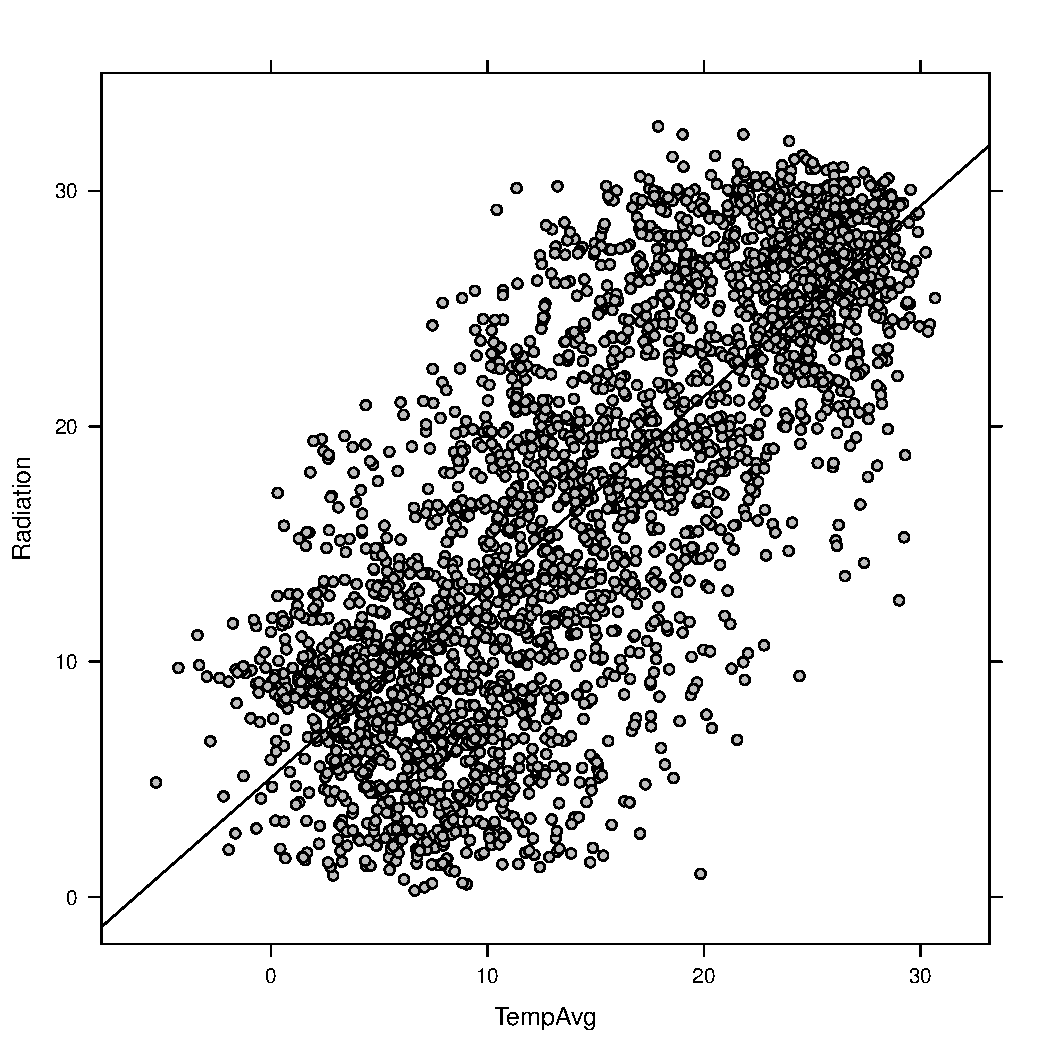
\includegraphics[height=0.6\textheight]{figs/intro.pdf}
\end{center}
\end{frame}

\section{Objetos en R}
\label{sec:org610de28}

\begin{frame}[fragile,label={sec:org33c73b1}]{Objetos en R}
 \begin{itemize}
\item Existen varios objetos en R:
\begin{itemize}
\item Vectores
\item Listas
\item Funciones
\item \ldots{}
\end{itemize}
\item A partir de estos objetos se definen varias clases:
\begin{itemize}
\item \texttt{matrix}
\item \texttt{data.frame}
\item \texttt{factor}
\item \texttt{Date}, \texttt{POSIXct}
\item \ldots{}
\end{itemize}
\end{itemize}
\end{frame}

\subsection{Vectores}
\label{sec:org0d43ef7}

\begin{frame}[fragile,label={sec:org5f70d74}]{Primeros pasos}
 \lstset{language=r,label= ,caption= ,captionpos=b,numbers=none}
\begin{lstlisting}
x <- 1:5
x
\end{lstlisting}

\begin{verbatim}
[1] 1 2 3 4 5
\end{verbatim}

\lstset{language=r,label= ,caption= ,captionpos=b,numbers=none}
\begin{lstlisting}
length(x)
\end{lstlisting}

\begin{verbatim}
[1] 5
\end{verbatim}

\lstset{language=r,label= ,caption= ,captionpos=b,numbers=none}
\begin{lstlisting}
class(x)
\end{lstlisting}

\begin{verbatim}
[1] "integer"
\end{verbatim}
\end{frame}


\begin{frame}[fragile,label={sec:orgfc4eb12}]{Generar vectores con \texttt{seq}}
 \lstset{language=r,label= ,caption= ,captionpos=b,numbers=none}
\begin{lstlisting}
x1 <- seq(1, 100, by=2)
x1
\end{lstlisting}

\begin{verbatim}
 [1]  1  3  5  7  9 11 13 15 17 19 21 23 25 27 29 31 33 35 37 39 41 43 45 47 49
[26] 51 53 55 57 59 61 63 65 67 69 71 73 75 77 79 81 83 85 87 89 91 93 95 97 99
\end{verbatim}

\lstset{language=r,label= ,caption= ,captionpos=b,numbers=none}
\begin{lstlisting}
seq(1, 100, length=10)
\end{lstlisting}

\begin{verbatim}
[1]   1  12  23  34  45  56  67  78  89 100
\end{verbatim}
\end{frame}


\begin{frame}[fragile,label={sec:orge9bd969}]{Unir vectores con \texttt{c}}
 \lstset{language=r,label= ,caption= ,captionpos=b,numbers=none}
\begin{lstlisting}
x <- c(1, 2, 3)
x
\end{lstlisting}

\begin{verbatim}
[1] 1 2 3
\end{verbatim}

\lstset{language=r,label= ,caption= ,captionpos=b,numbers=none}
\begin{lstlisting}
x <- seq(1, 100, length=10)
y <- seq(2, 100, length=50)
z <- c(x, y)
z
\end{lstlisting}

\begin{verbatim}
 [1]   1  12  23  34  45  56  67  78  89 100   2   4   6   8  10  12  14  16  18
[20]  20  22  24  26  28  30  32  34  36  38  40  42  44  46  48  50  52  54  56
[39]  58  60  62  64  66  68  70  72  74  76  78  80  82  84  86  88  90  92  94
[58]  96  98 100
\end{verbatim}
\end{frame}


\begin{frame}[fragile,label={sec:org134a348}]{Operaciones sencillas con vectores}
 \lstset{language=r,label= ,caption= ,captionpos=b,numbers=none}
\begin{lstlisting}
  x <- 1:5
  x + 1
\end{lstlisting}

\begin{verbatim}
[1] 2 3 4 5 6
\end{verbatim}

\lstset{language=r,label= ,caption= ,captionpos=b,numbers=none}
\begin{lstlisting}
  x^2
\end{lstlisting}

\begin{verbatim}
[1]  1  4  9 16 25
\end{verbatim}

\lstset{language=r,label= ,caption= ,captionpos=b,numbers=none}
\begin{lstlisting}
  y <- 1:10
  x + y
\end{lstlisting}

\begin{verbatim}
[1]  2  4  6  8 10  7  9 11 13 15
\end{verbatim}

\lstset{language=r,label= ,caption= ,captionpos=b,numbers=none}
\begin{lstlisting}
  x * y
\end{lstlisting}

\begin{verbatim}
[1]  1  4  9 16 25  6 14 24 36 50
\end{verbatim}

\lstset{language=r,label= ,caption= ,captionpos=b,numbers=none}
\begin{lstlisting}
  x^2 + y^3
\end{lstlisting}

\begin{verbatim}
[1]    2   12   36   80  150  217  347  521  745 1025
\end{verbatim}
\end{frame}




\begin{frame}[fragile,label={sec:orgb06fa53}]{Ejercicio}
 \begin{block}{Dibuja una circunferencia}
Sabiendo que la función \texttt{plot(x, y)} dibuja el vector \texttt{y} frente al
vector \texttt{x}, ¿qué código es necesario para dibujar una circunferencia
de un radio determinado?
\end{block}
\end{frame}


\subsection{Matrices}
\label{sec:org34ead66}
\begin{frame}[fragile,label={sec:org588df76}]{Construir una matriz}
 \lstset{language=r,label= ,caption= ,captionpos=b,numbers=none}
\begin{lstlisting}
  z <- 1:12
  M  <-  matrix(z, nrow=3)
  M
\end{lstlisting}

\begin{verbatim}
     [,1] [,2] [,3] [,4]
[1,]    1    4    7   10
[2,]    2    5    8   11
[3,]    3    6    9   12
\end{verbatim}

\lstset{language=r,label= ,caption= ,captionpos=b,numbers=none}
\begin{lstlisting}
  class(M)
\end{lstlisting}

\begin{verbatim}
[1] "matrix"
\end{verbatim}

\lstset{language=r,label= ,caption= ,captionpos=b,numbers=none}
\begin{lstlisting}
  dim(M)
\end{lstlisting}

\begin{verbatim}
[1] 3 4
\end{verbatim}

\lstset{language=r,label= ,caption= ,captionpos=b,numbers=none}
\begin{lstlisting}
  summary(M)
\end{lstlisting}

\begin{verbatim}
      V1            V2            V3            V4      
Min.   :1.0   Min.   :4.0   Min.   :7.0   Min.   :10.0  
1st Qu.:1.5   1st Qu.:4.5   1st Qu.:7.5   1st Qu.:10.5  
Median :2.0   Median :5.0   Median :8.0   Median :11.0  
Mean   :2.0   Mean   :5.0   Mean   :8.0   Mean   :11.0  
3rd Qu.:2.5   3rd Qu.:5.5   3rd Qu.:8.5   3rd Qu.:11.5  
Max.   :3.0   Max.   :6.0   Max.   :9.0   Max.   :12.0
\end{verbatim}
\end{frame}

\begin{frame}[fragile,label={sec:org7e5d8db}]{Matrices a partir de vectores: \texttt{rbind} y \texttt{cbind}}
 \lstset{language=r,label= ,caption= ,captionpos=b,numbers=none}
\begin{lstlisting}
z <- y <- x <- 1:10

M <- cbind(x, y, z)
M
\end{lstlisting}

\begin{verbatim}
       x  y  z
 [1,]  1  1  1
 [2,]  2  2  2
 [3,]  3  3  3
 [4,]  4  4  4
 [5,]  5  5  5
 [6,]  6  6  6
 [7,]  7  7  7
 [8,]  8  8  8
 [9,]  9  9  9
[10,] 10 10 10
\end{verbatim}

\lstset{language=r,label= ,caption= ,captionpos=b,numbers=none}
\begin{lstlisting}
M <- rbind(x, y, z)
M
\end{lstlisting}

\begin{verbatim}
  [,1] [,2] [,3] [,4] [,5] [,6] [,7] [,8] [,9] [,10]
x    1    2    3    4    5    6    7    8    9    10
y    1    2    3    4    5    6    7    8    9    10
z    1    2    3    4    5    6    7    8    9    10
\end{verbatim}
\end{frame}

\begin{frame}[fragile,label={sec:orgc851889}]{Álgebra matricial}
 \begin{description}
\item[{\texttt{t()}}] Transpuesta de una matriz
\item[{\texttt{*}}] Multiplicación elemento a elemento
\item[{\texttt{\%*\%}}] Multiplicación de matrices
\item[{\texttt{solve(A)}}] Inversa de una matriz (cuadrada)
\item \ldots{}
\end{description}
\end{frame}

\subsection{Listas}
\label{sec:org0b0b216}
\begin{frame}[fragile,label={sec:orgf0ced02}]{Para crear una lista usamos la función \texttt{list}}
 \lstset{language=r,label= ,caption= ,captionpos=b,numbers=none}
\begin{lstlisting}
lista <- list(a=c(1,3,5),
              b=c('l', 'p', 'r', 's'),
              c=3)
lista
\end{lstlisting}

\begin{verbatim}
$a
[1] 1 3 5

$b
[1] "l" "p" "r" "s"

$c
[1] 3
\end{verbatim}

\lstset{language=r,label= ,caption= ,captionpos=b,numbers=none}
\begin{lstlisting}
class(lista)
\end{lstlisting}

\begin{verbatim}
[1] "list"
\end{verbatim}

\lstset{language=r,label= ,caption= ,captionpos=b,numbers=none}
\begin{lstlisting}
length(lista)
\end{lstlisting}

\begin{verbatim}
[1] 3
\end{verbatim}
\end{frame}



\subsection{Data.frame}
\label{sec:orge6c545d}
\begin{frame}[fragile,label={sec:org3742b00}]{Para crear un \texttt{data.frame}\ldots{}}
 \lstset{language=r,label= ,caption= ,captionpos=b,numbers=none}
\begin{lstlisting}
  df <- data.frame(x = 1:5,
                   y = rnorm(10),
                   z = 0)
  df
\end{lstlisting}

\begin{verbatim}
   x           y z
1  1 -0.33032097 0
2  2  1.28167750 0
3  3  1.32421907 0
4  4  0.16471022 0
5  5  0.23235819 0
6  1 -0.60733133 0
7  2  0.21083478 0
8  3 -0.10171670 0
9  4  0.09755398 0
10 5  0.11925342 0
\end{verbatim}

\lstset{language=r,label= ,caption= ,captionpos=b,numbers=none}
\begin{lstlisting}
  length(df)
\end{lstlisting}

\begin{verbatim}
[1] 3
\end{verbatim}

\lstset{language=r,label= ,caption= ,captionpos=b,numbers=none}
\begin{lstlisting}
  dim(df)
\end{lstlisting}

\begin{verbatim}
[1] 10  3
\end{verbatim}
\end{frame}

\begin{frame}[fragile,label={sec:orga5edc36}]{A partir de ficheros}
 \lstset{language=r,label= ,caption= ,captionpos=b,numbers=none}
\begin{lstlisting}
dats <- read.table('data/aranjuez.csv',
                   sep=',',
                   header=TRUE)
\end{lstlisting}

\lstset{language=r,label= ,caption= ,captionpos=b,numbers=none}
\begin{lstlisting}
head(dats)
\end{lstlisting}

\begin{verbatim}
           X TempAvg TempMax TempMin HumidAvg HumidMax WindAvg WindMax Rain
1 2004-01-01   4.044   10.71  -1.969     88.3     95.9   0.746   3.528    0
2 2004-01-02   5.777   11.52   1.247     83.3     98.5   1.078   6.880    0
3 2004-01-03   5.850   13.32   0.377     75.0     94.4   0.979   6.576    0
4 2004-01-04   4.408   15.59  -2.576     82.0     97.0   0.633   3.704    0
5 2004-01-05   3.081   14.58  -2.974     83.2     97.0   0.389   2.244    0
6 2004-01-06   2.304   11.83  -3.379     84.5     96.5   0.436   2.136    0
  Radiation        ET
1     5.490 0.5352688
2     6.537 0.7710499
3     8.810 0.8361229
4     9.790 0.6861381
5    10.300 0.5152422
6     9.940 0.4886631
\end{verbatim}

\alert{Atención: usa \texttt{setwd} para configurar ruta}
\end{frame}

\begin{frame}[fragile,label={sec:org9e195da}]{A partir de ficheros remotos}
 \lstset{language=r,label= ,caption= ,captionpos=b,numbers=none}
\begin{lstlisting}
remoto <- read.table('https://raw.githubusercontent.com/oscarperpinan/R/master/data/aranjuez.csv',
                     sep=',',
                     header=TRUE)
\end{lstlisting}

\lstset{language=r,label= ,caption= ,captionpos=b,numbers=none}
\begin{lstlisting}
head(remoto)
\end{lstlisting}

\begin{verbatim}
           X TempAvg TempMax TempMin HumidAvg HumidMax WindAvg WindMax Rain
1 2004-01-01   4.044   10.71  -1.969     88.3     95.9   0.746   3.528    0
2 2004-01-02   5.777   11.52   1.247     83.3     98.5   1.078   6.880    0
3 2004-01-03   5.850   13.32   0.377     75.0     94.4   0.979   6.576    0
4 2004-01-04   4.408   15.59  -2.576     82.0     97.0   0.633   3.704    0
5 2004-01-05   3.081   14.58  -2.974     83.2     97.0   0.389   2.244    0
6 2004-01-06   2.304   11.83  -3.379     84.5     96.5   0.436   2.136    0
  Radiation        ET
1     5.490 0.5352688
2     6.537 0.7710499
3     8.810 0.8361229
4     9.790 0.6861381
5    10.300 0.5152422
6     9.940 0.4886631
\end{verbatim}

\lstset{language=r,label= ,caption= ,captionpos=b,numbers=none}
\begin{lstlisting}
identical(dats, remoto)
\end{lstlisting}

\begin{verbatim}
[1] TRUE
\end{verbatim}
\end{frame}


\begin{frame}[fragile,label={sec:org9cf788e}]{Ejercicio}
 \begin{block}{Dibuja una circunferencia}
¿Qué código hay que emplear para dibujar una circunferencia de forma
que todos los vectores implicados sean columnas de un \texttt{data.frame}?
\end{block}
\end{frame}


\section{Indexado}
\label{sec:orgd9c1ecf}

\subsection{Condiciones lógicas}
\label{sec:org699240b}
\begin{frame}[fragile,label={sec:orgaf4b259}]{Condiciones simples}
 \lstset{language=r,label= ,caption= ,captionpos=b,numbers=none}
\begin{lstlisting}
x <- seq(-1, 1, .1)
x
\end{lstlisting}

\begin{verbatim}
 [1] -1.0 -0.9 -0.8 -0.7 -0.6 -0.5 -0.4 -0.3 -0.2 -0.1  0.0  0.1  0.2  0.3  0.4
[16]  0.5  0.6  0.7  0.8  0.9  1.0
\end{verbatim}

\lstset{language=r,label= ,caption= ,captionpos=b,numbers=none}
\begin{lstlisting}
x < 0
\end{lstlisting}

\begin{verbatim}
 [1]  TRUE  TRUE  TRUE  TRUE  TRUE  TRUE  TRUE  TRUE  TRUE  TRUE FALSE FALSE
[13] FALSE FALSE FALSE FALSE FALSE FALSE FALSE FALSE FALSE
\end{verbatim}

\lstset{language=r,label= ,caption= ,captionpos=b,numbers=none}
\begin{lstlisting}
x >= 0
\end{lstlisting}

\begin{verbatim}
 [1] FALSE FALSE FALSE FALSE FALSE FALSE FALSE FALSE FALSE FALSE  TRUE  TRUE
[13]  TRUE  TRUE  TRUE  TRUE  TRUE  TRUE  TRUE  TRUE  TRUE
\end{verbatim}

\lstset{language=r,label= ,caption= ,captionpos=b,numbers=none}
\begin{lstlisting}
x == 0
\end{lstlisting}

\begin{verbatim}
 [1] FALSE FALSE FALSE FALSE FALSE FALSE FALSE FALSE FALSE FALSE  TRUE FALSE
[13] FALSE FALSE FALSE FALSE FALSE FALSE FALSE FALSE FALSE
\end{verbatim}

\lstset{language=r,label= ,caption= ,captionpos=b,numbers=none}
\begin{lstlisting}
x != 0
\end{lstlisting}

\begin{verbatim}
 [1]  TRUE  TRUE  TRUE  TRUE  TRUE  TRUE  TRUE  TRUE  TRUE  TRUE FALSE  TRUE
[13]  TRUE  TRUE  TRUE  TRUE  TRUE  TRUE  TRUE  TRUE  TRUE
\end{verbatim}
\end{frame}

\begin{frame}[fragile,label={sec:org404979d}]{Condiciones múltiples}
 \lstset{language=r,label= ,caption= ,captionpos=b,numbers=none}
\begin{lstlisting}
cond  <-  (x > 0) & (x < .5)
cond
\end{lstlisting}

\begin{verbatim}
 [1] FALSE FALSE FALSE FALSE FALSE FALSE FALSE FALSE FALSE FALSE FALSE  TRUE
[13]  TRUE  TRUE  TRUE FALSE FALSE FALSE FALSE FALSE FALSE
\end{verbatim}

\lstset{language=r,label= ,caption= ,captionpos=b,numbers=none}
\begin{lstlisting}
cond  <-  (x >= .5) | (x <= -.5)
cond
\end{lstlisting}

\begin{verbatim}
 [1]  TRUE  TRUE  TRUE  TRUE  TRUE  TRUE FALSE FALSE FALSE FALSE FALSE FALSE
[13] FALSE FALSE FALSE  TRUE  TRUE  TRUE  TRUE  TRUE  TRUE
\end{verbatim}
\end{frame}


\begin{frame}[fragile,label={sec:org50a69fb}]{Con las condiciones se pueden hacer operaciones}
 \lstset{language=r,label= ,caption= ,captionpos=b,numbers=none}
\begin{lstlisting}
sum(cond)
\end{lstlisting}

\begin{verbatim}
[1] 12
\end{verbatim}

\lstset{language=r,label= ,caption= ,captionpos=b,numbers=none}
\begin{lstlisting}
sum(!cond)
\end{lstlisting}

\begin{verbatim}
[1] 9
\end{verbatim}

\lstset{language=r,label= ,caption= ,captionpos=b,numbers=none}
\begin{lstlisting}
as.numeric(cond)
\end{lstlisting}

\begin{verbatim}
[1] 1 1 1 1 1 1 0 0 0 0 0 0 0 0 0 1 1 1 1 1 1
\end{verbatim}
\end{frame}


\subsection{Vectores}
\label{sec:org1692bbc}
\begin{frame}[fragile,label={sec:org9369186}]{Indexado numérico}
 \lstset{language=r,label= ,caption= ,captionpos=b,numbers=none}
\begin{lstlisting}
  x <- seq(1, 100, 2)
  x
\end{lstlisting}

\begin{verbatim}
 [1]  1  3  5  7  9 11 13 15 17 19 21 23 25 27 29 31 33 35 37 39 41 43 45 47 49
[26] 51 53 55 57 59 61 63 65 67 69 71 73 75 77 79 81 83 85 87 89 91 93 95 97 99
\end{verbatim}

\lstset{language=r,label= ,caption= ,captionpos=b,numbers=none}
\begin{lstlisting}
  x[1:5]
\end{lstlisting}

\begin{verbatim}
[1] 1 3 5 7 9
\end{verbatim}

\lstset{language=r,label= ,caption= ,captionpos=b,numbers=none}
\begin{lstlisting}
  x[10:5]
\end{lstlisting}

\begin{verbatim}
[1] 19 17 15 13 11  9
\end{verbatim}
\end{frame}

\begin{frame}[fragile,label={sec:orga754310}]{Indexado con condiciones lógicas}
 \lstset{language=r,label= ,caption= ,captionpos=b,numbers=none}
\begin{lstlisting}
  x[x != 9]
\end{lstlisting}

\begin{verbatim}
 [1]  1  3  5  7 11 13 15 17 19 21 23 25 27 29 31 33 35 37 39 41 43 45 47 49 51
[26] 53 55 57 59 61 63 65 67 69 71 73 75 77 79 81 83 85 87 89 91 93 95 97 99
\end{verbatim}

\lstset{language=r,label= ,caption= ,captionpos=b,numbers=none}
\begin{lstlisting}
  x[x > 20]
\end{lstlisting}

\begin{verbatim}
 [1] 21 23 25 27 29 31 33 35 37 39 41 43 45 47 49 51 53 55 57 59 61 63 65 67 69
[26] 71 73 75 77 79 81 83 85 87 89 91 93 95 97 99
\end{verbatim}

\lstset{language=r,label= ,caption= ,captionpos=b,numbers=none}
\begin{lstlisting}
x[x %in% seq(0, 10, .5)]
\end{lstlisting}

\begin{verbatim}
[1] 1 3 5 7 9
\end{verbatim}
\end{frame}

\begin{frame}[fragile,label={sec:org3bb5368}]{Indexado con condiciones múltiples}
 \lstset{language=r,label= ,caption= ,captionpos=b,numbers=none}
\begin{lstlisting}
z <- seq(-10, 10, by = .5)
z
\end{lstlisting}

\begin{verbatim}
 [1] -10.0  -9.5  -9.0  -8.5  -8.0  -7.5  -7.0  -6.5  -6.0  -5.5  -5.0  -4.5
[13]  -4.0  -3.5  -3.0  -2.5  -2.0  -1.5  -1.0  -0.5   0.0   0.5   1.0   1.5
[25]   2.0   2.5   3.0   3.5   4.0   4.5   5.0   5.5   6.0   6.5   7.0   7.5
[37]   8.0   8.5   9.0   9.5  10.0
\end{verbatim}

\lstset{language=r,label= ,caption= ,captionpos=b,numbers=none}
\begin{lstlisting}
z[z < -5 | z > 5]
\end{lstlisting}

\begin{verbatim}
 [1] -10.0  -9.5  -9.0  -8.5  -8.0  -7.5  -7.0  -6.5  -6.0  -5.5   5.5   6.0
[13]   6.5   7.0   7.5   8.0   8.5   9.0   9.5  10.0
\end{verbatim}

\lstset{language=r,label= ,caption= ,captionpos=b,numbers=none}
\begin{lstlisting}
cond <- (z >= 0 & z <= 5)
cond
\end{lstlisting}

\begin{verbatim}
 [1] FALSE FALSE FALSE FALSE FALSE FALSE FALSE FALSE FALSE FALSE FALSE FALSE
[13] FALSE FALSE FALSE FALSE FALSE FALSE FALSE FALSE  TRUE  TRUE  TRUE  TRUE
[25]  TRUE  TRUE  TRUE  TRUE  TRUE  TRUE  TRUE FALSE FALSE FALSE FALSE FALSE
[37] FALSE FALSE FALSE FALSE FALSE
\end{verbatim}

\lstset{language=r,label= ,caption= ,captionpos=b,numbers=none}
\begin{lstlisting}
z[cond]
\end{lstlisting}

\begin{verbatim}
[1] 0.0 0.5 1.0 1.5 2.0 2.5 3.0 3.5 4.0 4.5 5.0
\end{verbatim}
\end{frame}

\subsection{Matrices}
\label{sec:orgb5aad98}
\begin{frame}[fragile,label={sec:orgb958d04}]{Indexado de matrices}
 \lstset{language=r,label= ,caption= ,captionpos=b,numbers=none}
\begin{lstlisting}
M[1:2, ]
\end{lstlisting}

\begin{verbatim}
  [,1] [,2] [,3] [,4] [,5] [,6] [,7] [,8] [,9] [,10]
x    1    2    3    4    5    6    7    8    9    10
y    1    2    3    4    5    6    7    8    9    10
\end{verbatim}

\lstset{language=r,label= ,caption= ,captionpos=b,numbers=none}
\begin{lstlisting}
M[1:2, 2:3]
\end{lstlisting}

\begin{verbatim}
  [,1] [,2]
x    2    3
y    2    3
\end{verbatim}

\lstset{language=r,label= ,caption= ,captionpos=b,numbers=none}
\begin{lstlisting}
M[1, c(1, 4)]
\end{lstlisting}

\begin{verbatim}
[1] 1 4
\end{verbatim}
\end{frame}

\begin{frame}[fragile,label={sec:orga2128ec}]{Indexado de matrices}
 \lstset{language=r,label= ,caption= ,captionpos=b,numbers=none}
\begin{lstlisting}
M[-1,]
\end{lstlisting}

\begin{verbatim}
  [,1] [,2] [,3] [,4] [,5] [,6] [,7] [,8] [,9] [,10]
y    1    2    3    4    5    6    7    8    9    10
z    1    2    3    4    5    6    7    8    9    10
\end{verbatim}

\lstset{language=r,label= ,caption= ,captionpos=b,numbers=none}
\begin{lstlisting}
M[-c(1, 2),]
\end{lstlisting}

\begin{verbatim}
[1]  1  2  3  4  5  6  7  8  9 10
\end{verbatim}
\end{frame}

\subsection{Listas}
\label{sec:orgda01168}
\begin{frame}[fragile,label={sec:org2a4192c}]{Podemos acceder a los elementos\ldots{}}
 \begin{itemize}
\item Por su nombre
\end{itemize}
\lstset{language=r,label= ,caption= ,captionpos=b,numbers=none}
\begin{lstlisting}
lista$a
\end{lstlisting}

\begin{verbatim}
[1] 1 3 5
\end{verbatim}

\begin{itemize}
\item o por su índice
\end{itemize}
\lstset{language=r,label= ,caption= ,captionpos=b,numbers=none}
\begin{lstlisting}
  lista[1]
\end{lstlisting}

\begin{verbatim}
$a
[1] 1 3 5
\end{verbatim}

\lstset{language=r,label= ,caption= ,captionpos=b,numbers=none}
\begin{lstlisting}
  lista[[1]]
\end{lstlisting}

\begin{verbatim}
[1] 1 3 5
\end{verbatim}
\end{frame}


\subsection{Data Frame}
\label{sec:org820258a}
\begin{frame}[fragile,label={sec:orgd35cb22}]{Podemos acceder a los elementos}
 \lstset{language=r,label= ,caption= ,captionpos=b,numbers=none}
\begin{lstlisting}
  df <- data.frame(x = 1:5,
                   y = rnorm(10),
                   z = 0)
\end{lstlisting}

\begin{itemize}
\item Por su nombre (como una lista)
\end{itemize}
\lstset{language=r,label= ,caption= ,captionpos=b,numbers=none}
\begin{lstlisting}
df$x
\end{lstlisting}

\begin{verbatim}
[1] 1 2 3 4 5 1 2 3 4 5
\end{verbatim}

\begin{itemize}
\item Por su índice (como una matriz)
\end{itemize}
\lstset{language=r,label= ,caption= ,captionpos=b,numbers=none}
\begin{lstlisting}
df[1,]
\end{lstlisting}

\begin{verbatim}
  x         y z
1 1 0.4638927 0
\end{verbatim}

\lstset{language=r,label= ,caption= ,captionpos=b,numbers=none}
\begin{lstlisting}
df[,1]
\end{lstlisting}

\begin{verbatim}
[1] 1 2 3 4 5 1 2 3 4 5
\end{verbatim}
\end{frame}

\begin{frame}[fragile,label={sec:orgc13df22}]{Indexado lógico}
 \begin{itemize}
\item Hay que explicitar dos veces el \texttt{data.frame}:
\end{itemize}
\lstset{language=r,label= ,caption= ,captionpos=b,numbers=none}
\begin{lstlisting}
df[df$y > 0,]
\end{lstlisting}

\begin{verbatim}
   x         y z
1  1 0.4638927 0
3  3 1.7401387 0
4  4 0.8324874 0
10 5 0.7390417 0
\end{verbatim}

\begin{itemize}
\item La función \texttt{subset} simplifica el código:
\end{itemize}
\lstset{language=r,label= ,caption= ,captionpos=b,numbers=none}
\begin{lstlisting}
subset(df, y > 0)
\end{lstlisting}

\begin{verbatim}
   x         y z
1  1 0.4638927 0
3  3 1.7401387 0
4  4 0.8324874 0
10 5 0.7390417 0
\end{verbatim}
\end{frame}

\begin{frame}[fragile,label={sec:org6a2203e}]{Uso de \texttt{with}}
 \begin{itemize}
\item Problema: el código con varias variables puede ser ilegible
\end{itemize}
\lstset{language=r,label= ,caption= ,captionpos=b,numbers=none}
\begin{lstlisting}
df$x^2 + df$y^2
\end{lstlisting}
\begin{itemize}
\item La función \texttt{with} permite acceder a varias variables con una única llamada:
\end{itemize}
\lstset{language=r,label= ,caption= ,captionpos=b,numbers=none}
\begin{lstlisting}
with(df, x^2 + y^2)
\end{lstlisting}

\begin{verbatim}
[1]  1.215196  9.081672 12.028083 16.693035 25.228874  1.000037  4.942512
[8] 13.679944 16.082390 25.546183
\end{verbatim}

\lstset{language=r,label= ,caption= ,captionpos=b,numbers=none}
\begin{lstlisting}
with(df, x[y > 0])
\end{lstlisting}

\begin{verbatim}
[1] 1 3 4 5
\end{verbatim}
\end{frame}

\section{Funciones}
\label{sec:org9d31787}
\subsection{Definición de funciones}
\label{sec:org6c45123}
\begin{frame}[fragile,label={sec:org2792f02}]{Componentes de una función}
 \begin{itemize}
\item Una función se define con \texttt{function}
\end{itemize}
\begin{center}
\texttt{name <- function(arg\_1, arg\_2, ...) expression}
\end{center}
\begin{itemize}
\item Está compuesta por:
\begin{itemize}
\item Nombre de la función (\texttt{name})
\item Argumentos (\texttt{arg\_1}, \texttt{arg\_2}, \texttt{...})
\item Cuerpo (\texttt{expression}): emplea los argumentos para generar un resultado
\end{itemize}
\end{itemize}
\end{frame}


\begin{frame}[fragile,label={sec:org1a42eae}]{Argumentos: nombre y orden}
 Una función identifica sus argumentos por su nombre y por su orden (sin nombre)

\lstset{language=r,label= ,caption= ,captionpos=b,numbers=none}
\begin{lstlisting}
eleva <- function(x, p)
{
    x ^ p
}
\end{lstlisting}

\lstset{language=r,label= ,caption= ,captionpos=b,numbers=none}
\begin{lstlisting}
eleva(x = 1:10, p = 2)
\end{lstlisting}

\begin{verbatim}
[1]   1   4   9  16  25  36  49  64  81 100
\end{verbatim}

\lstset{language=r,label= ,caption= ,captionpos=b,numbers=none}
\begin{lstlisting}
eleva(1:10, p = 2)
\end{lstlisting}

\begin{verbatim}
[1]   1   4   9  16  25  36  49  64  81 100
\end{verbatim}

\lstset{language=r,label= ,caption= ,captionpos=b,numbers=none}
\begin{lstlisting}
eleva(p = 2, x = 1:10)
\end{lstlisting}

\begin{verbatim}
[1]   1   4   9  16  25  36  49  64  81 100
\end{verbatim}
\end{frame}

\begin{frame}[fragile,label={sec:org418bb9a}]{Argumentos: valores por defecto}
 \begin{itemize}
\item Se puede asignar un valor por defecto a los argumentos
\end{itemize}
\lstset{language=r,label= ,caption= ,captionpos=b,numbers=none}
\begin{lstlisting}
eleva <- function(x, p = 2)
{
    x ^ p
}
\end{lstlisting}

\lstset{language=r,label= ,caption= ,captionpos=b,numbers=none}
\begin{lstlisting}
eleva(1:10)
\end{lstlisting}

\begin{verbatim}
[1]   1   4   9  16  25  36  49  64  81 100
\end{verbatim}

\lstset{language=r,label= ,caption= ,captionpos=b,numbers=none}
\begin{lstlisting}
eleva(1:10, 2)
\end{lstlisting}

\begin{verbatim}
[1]   1   4   9  16  25  36  49  64  81 100
\end{verbatim}
\end{frame}

\begin{frame}[fragile,label={sec:org062ccb0}]{Argumentos sin nombre: \texttt{...}}
 \lstset{language=r,label= ,caption= ,captionpos=b,numbers=none}
\begin{lstlisting}
pwrSum <- function(x, p, ...)
{
    sum(x ^ p, ...)
}
\end{lstlisting}

\lstset{language=r,label= ,caption= ,captionpos=b,numbers=none}
\begin{lstlisting}
x <- 1:10
pwrSum(x, 2)
\end{lstlisting}

\begin{verbatim}
[1] 385
\end{verbatim}

\lstset{language=r,label= ,caption= ,captionpos=b,numbers=none}
\begin{lstlisting}
x <- c(1:5, NA, 6:9, NA, 10)
pwrSum(x, 2)
\end{lstlisting}

\begin{verbatim}
[1] NA
\end{verbatim}

\lstset{language=r,label= ,caption= ,captionpos=b,numbers=none}
\begin{lstlisting}
pwrSum(x, 2, na.rm=TRUE)
\end{lstlisting}

\begin{verbatim}
[1] 385
\end{verbatim}
\end{frame}

\begin{frame}[fragile,label={sec:org340ed79}]{Podemos construir a partir de funciones}
 \lstset{language=r,label= ,caption= ,captionpos=b,numbers=none}
\begin{lstlisting}
foo  <-  function(x, ...){
  mx <- mean(x, ...)
  medx <- median(x, ...)
  sdx <- sd(x, ...)
  c(mx, medx, sdx)
  }
\end{lstlisting}

\lstset{language=r,label= ,caption= ,captionpos=b,numbers=none}
\begin{lstlisting}
foo(1:10)
\end{lstlisting}

\begin{verbatim}
[1] 5.50000 5.50000 3.02765
\end{verbatim}

\lstset{language=r,label= ,caption= ,captionpos=b,numbers=none}
\begin{lstlisting}
foo(rnorm(1e5))
\end{lstlisting}

\begin{verbatim}
[1] 0.001531192 0.001289880 1.001371477
\end{verbatim}
\end{frame}

\begin{frame}[fragile,label={sec:org430984a}]{Ejercicio}
 \begin{block}{Dibuja una circunferencia}
Define una función de dos argumentos, \texttt{theta} (vector de ángulos) y
\texttt{r} (radio), que entregue un \texttt{data.frame} de dos columnas, \texttt{x} e \texttt{y},
con las coordenadas del arco de circunferencia que corresponde a los
argumentos de la función, y emplea esta función para dibujar una
circunferencia completa.
\end{block}
\end{frame}


\subsection{Funciones predefinidas}
\label{sec:org2401417}

\begin{frame}[fragile,label={sec:orgfcd5ee0}]{Funciones en paquetes}
 \begin{itemize}
\item \texttt{R} proporciona un amplio conjunto de funciones predefinidas agrupadas en paquetes

\begin{itemize}
\item Algunos paquetes vienen instalados y se cargan al empezar (\emph{base}):
\end{itemize}
\end{itemize}
\lstset{language=r,label= ,caption= ,captionpos=b,numbers=none}
\begin{lstlisting}
  sessionInfo()
\end{lstlisting}
\begin{itemize}
\item Otros vienen instalados pero hay que cargarlos (\emph{recommended}):
\end{itemize}
\lstset{language=r,label= ,caption= ,captionpos=b,numbers=none}
\begin{lstlisting}
  library(lattice)

  packageDescription('lattice')
\end{lstlisting}
\begin{itemize}
\item Otros hay que instalarlos y después cargarlos (\emph{contributed}):
\end{itemize}
\lstset{language=r,label= ,caption= ,captionpos=b,numbers=none}
\begin{lstlisting}
  install.packages('data.table')
\end{lstlisting}

\lstset{language=r,label= ,caption= ,captionpos=b,numbers=none}
\begin{lstlisting}
  library('data.table')
  packageDescription('data.table')
\end{lstlisting}
\end{frame}

\section{Bucles}
\label{sec:org72dab04}
\subsection{Matrices}
\label{sec:org75de290}
\begin{frame}[fragile,label={sec:org8b62386}]{La función \texttt{apply}}
 \lstset{language=r,label= ,caption= ,captionpos=b,numbers=none}
\begin{lstlisting}
apply(M, 1, sum)
\end{lstlisting}

\begin{verbatim}
 x  y  z 
55 55 55
\end{verbatim}

\lstset{language=r,label= ,caption= ,captionpos=b,numbers=none}
\begin{lstlisting}
rowSums(M)
\end{lstlisting}

\begin{verbatim}
 x  y  z 
55 55 55
\end{verbatim}

\lstset{language=r,label= ,caption= ,captionpos=b,numbers=none}
\begin{lstlisting}
apply(M, 2, mean)
\end{lstlisting}

\begin{verbatim}
[1]  1  2  3  4  5  6  7  8  9 10
\end{verbatim}

\lstset{language=r,label= ,caption= ,captionpos=b,numbers=none}
\begin{lstlisting}
colMeans(M)
\end{lstlisting}

\begin{verbatim}
[1]  1  2  3  4  5  6  7  8  9 10
\end{verbatim}
\end{frame}

\subsection{Listas / \texttt{data.frame}}
\label{sec:org614354e}
\begin{frame}[fragile,label={sec:orgdaadcf3}]{\texttt{lapply} y \texttt{sapply}}
 \lstset{language=r,label= ,caption= ,captionpos=b,numbers=none}
\begin{lstlisting}
lista <- list(x = 1:10,
              y = seq(0, 10, 2),
              z = rnorm(30))
lapply(lista, sum)
\end{lstlisting}

\begin{verbatim}
$x
[1] 55

$y
[1] 30

$z
[1] 10.17344
\end{verbatim}

\lstset{language=r,label= ,caption= ,captionpos=b,numbers=none}
\begin{lstlisting}
sapply(lista, sum)
\end{lstlisting}

\begin{verbatim}
       x        y        z 
55.00000 30.00000 10.17344
\end{verbatim}
\end{frame}

\begin{frame}[fragile,label={sec:orga122d1d}]{Ejercicio}
 \begin{block}{}
\begin{itemize}
\item Calcula la media de cada una de las columnas de \texttt{remoto}.
\item Calcula la media, mediana y desviación estándar de cada una de las columnas de \texttt{remoto}.
\item Calcula la media de los valores positivos de cada una de las columnas de \texttt{remoto}.
\end{itemize}
\end{block}

\begin{block}{}
\lstset{language=r,label= ,caption= ,captionpos=b,numbers=none}
\begin{lstlisting}
remoto <- read.csv('https://raw.githubusercontent.com/oscarperpinan/R/master/data/aranjuez.csv')
\end{lstlisting}
\end{block}
\end{frame}


\subsection{Bucles \texttt{for}}
\label{sec:org7b10f89}
\begin{frame}[fragile,label={sec:org760fe10}]{\texttt{for}}
 \begin{itemize}
\item En \texttt{R} suele usarse más la familia de funciones \texttt{*apply} con funciones vectorizadas.
\item No obstante, \texttt{for} puede tener su utilidad:
\end{itemize}
\lstset{language=r,label= ,caption= ,captionpos=b,numbers=none}
\begin{lstlisting}
for(n in c(2,5,10,20,50)) {
    x <- rnorm(n)
    cat(n,":", sum(x^2),"\n")
}
\end{lstlisting}

\begin{verbatim}
2 : 0.1992612 
5 : 12.71815 
10 : 5.001255 
20 : 13.64171 
50 : 45.56089
\end{verbatim}
\end{frame}

\subsection{Condiciones con \texttt{if}, \texttt{else} e \texttt{ifelse}}
\label{sec:org33b7abd}
\begin{frame}[fragile,label={sec:org24919c0}]{\texttt{if}}
 \begin{itemize}
\item En \texttt{R} suele usarse más el indexado lógico (vectorizado).
\item ¿Cuál es el equivalente a este bucle for-if?
\end{itemize}
\lstset{language=r,label= ,caption= ,captionpos=b,numbers=none}
\begin{lstlisting}
  x <- rnorm(10)
  x2 <- numeric(length(x))
  for (i in seq_along(x2)){
      if (x[i]<0) x2[i] <- 0 else x2[i] <- 1
      }
  cbind(x, x2)
\end{lstlisting}

\begin{verbatim}
               x x2
 [1,]  1.0000731  1
 [2,]  0.3611223  1
 [3,] -0.5802274  0
 [4,]  2.7501777  1
 [5,]  1.3758549  1
 [6,] -0.6449127  0
 [7,] -2.3812881  0
 [8,]  1.2498486  1
 [9,] -0.6768266  0
[10,]  1.1902771  1
\end{verbatim}
\end{frame}

\begin{frame}[fragile,label={sec:orga8757eb}]{\texttt{ifelse}}
 \lstset{language=r,label= ,caption= ,captionpos=b,numbers=none}
\begin{lstlisting}
x <- rnorm(10)
x
\end{lstlisting}

\begin{verbatim}
[1]  0.2304201 -1.2034347  1.4732810 -0.1425186 -1.5511399 -1.9353629
[7] -0.3620471  1.3926926 -0.5778959 -0.4644164
\end{verbatim}

\lstset{language=r,label= ,caption= ,captionpos=b,numbers=none}
\begin{lstlisting}
ifelse(x>0, 1, 0)
\end{lstlisting}

\begin{verbatim}
[1] 1 0 1 0 0 0 0 1 0 0
\end{verbatim}
\end{frame}
\end{document}